\documentclass{beamer}

\usepackage{beamerthemesplit}
\usepackage{graphicx}
\DeclareGraphicsRule{*}{mps}{*}{}

\usetheme{Warsaw}
\setbeamercovered{transparent}

\title{TreeFam: Updates and Algorithms}
\author{Heng Li}
\institute[inst]{Beijing Genomics Institute, CAS\\
Institute of Theoretical Physics, CAS}
\date{March 17, 2006}

\begin{document}

\frame{\titlepage}

\AtBeginSection[]{\frame{\frametitle{Outline}\tableofcontents[current]}}
\part{Main Part}

\frame{\frametitle{Outline}\tableofcontents[part=1]}

\section{TreeFam Update}
\subsection{Status}
\frame {
	\frametitle{Status}
	\begin{itemize}
		\item 19 Speices: 10 vertebrates (5 mammals), {\it Ciona}, 3 insects, 2 worms, 3 outgroups
		\item Number of family-A: 1166
		\item Number of family-B: 15262, but about one third of them contain no vertebrate sequences or only consist of 2 or 3 sequences.
		\item Gene coverage: human 93.6\%, {\it Drosophila} 79.7\%, {\it C. elegans} 83.8\%
	\end{itemize}
}
\subsection{Parameter Changes}
\frame {
	\frametitle{Parameter Changes}
	\begin{itemize}
		\item BLAST E-value cutoff: \alert{0.01} (previous $1e-5$)
		\item HMMER E-value cutoff: \alert{0.1} (previous $10$)
		\item MUSCLE: exhaustive mode (in TreeFam-3.0)
	\end{itemize}
}
\subsection{Clustering PhIGs}
\frame {
	\frametitle{Clustering PhIGs: Problems with PhIGs clusters}
	\begin{itemize}
		\item PhIGs clusters are too tight.
		\item Subfamilies are frequently encountered.
	\end{itemize}
}
\frame {
	\frametitle{Clustering PhIGs}
	\begin{itemize}
		\item Given PhIGs cluster $u$, let $R_u\in u$ be the set of animal genes whose
			HMMER bit-scores are higher than scores of any outgroup genes in $u$.
		\item An edge $[u,v]$ is added if $R_u\cap R_v\not=\emptyset$.
		\item Weight $w_{uv}=\frac{|R_u\cap R_v|}{\min\{|R_u|,|R_v|\}}$.
		\item Find groups in which edges tend to be saturated.
		\item Only one round is applied.
	\end{itemize}
}
\frame {
	\frametitle{Clustering PhIGs: Problems and Suggestions}
	\begin{itemize}
		\item In fact, MCL algorithm is the more sophisticated one.
		\item Remaining \alert{problem}: some subfamilies still exist.
		\item Suggestion: build clusters by ourselves?
	\end{itemize}
}
\subsection{Competitive Method}
\frame {
	\frametitle{Competitive Method: Problems with TreeFam-1.x}
	\begin{itemize}
		\item One gene belongs to several families because:
		\begin{itemize}
			\item A PhIGs cluster sometimes represents a subfamily.
			\item Long branches are hard to be resolved correctly, which affects tree-cutting.
		\end{itemize}
		\item Aggregate computational burden.
	\end{itemize}
}
\frame {
	\frametitle{Competitive Method: Method and Problems}
	\begin{itemize}
		\item One sequence is arbitrarily assigned to one family. One gene can be present
				in several.
		\item Usually work well if the quality of seeds is high enough.
		\item Remaining \alert{problems}:
			\begin{itemize}
			\item When seed contains few sequences or the seed alignment is too poor, HMMER scores
					become inaccurate.
			\item Even if a gene does not belong to any existing TreeFam families, it will still be forced to be
					assigned no matter how low the BLAST and HMMER scores are. (Examples in next page)
			\end{itemize}
	\end{itemize}
}
\frame {
	\frametitle{Competitive Method: Example 1}
	{\center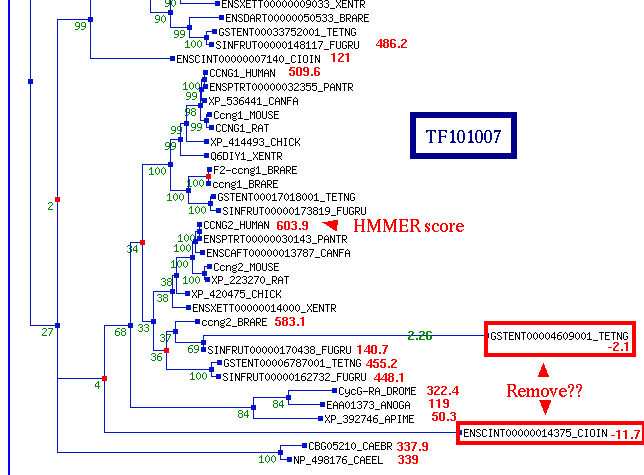
\includegraphics[height=7cm]{example-1.png}}
}
\frame {
	\frametitle{Competitive Method: Example 2}
	{\center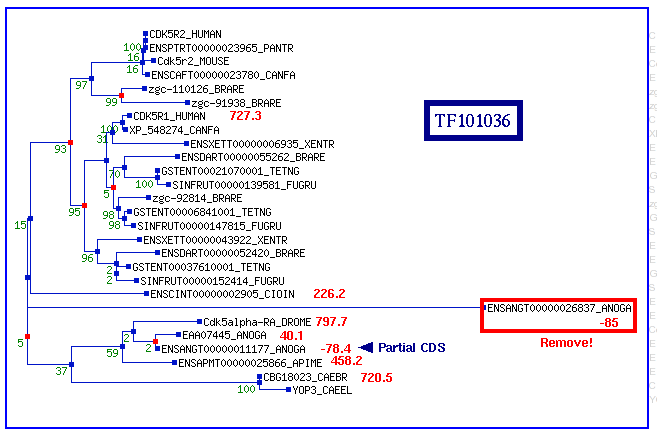
\includegraphics[height=7cm]{example-2.png}}
}
\frame {
	\frametitle{Competitive Method: Possible Solutions}
	\begin{itemize}
		\item Solution:
			\begin{itemize}
			\item Leave the problem as it is. Only discard weird genes in seed trees.
			\item Automatically detect them before building the trees (by sequence similarity,
					branch length and hmmer score)
			\end{itemize}
		\item Warnings:
			\begin{itemize}
			\item HMMER score alone is not a good standard (example 2).
			\item Mis-annotated exons and gene fusions interfere sometimes.
			\end{itemize}
	\end{itemize}
}
\subsection{Tracing Identifiers}
\frame {
	\frametitle{Tracing Identifiers}
	\begin{itemize}
		\item Importance: reserve curation information
		\item A new identifier can be mapped to an old one if:
		\begin{itemize}
			\item The two sequences come from the same species.
			\item They are almost identical in matched regions.
			\item No other sequence is closer to either of them.
		\end{itemize}
		\item Method: Build a tree that consists of both unchanged sequences and
			sequences whose identifiers are only present in one release.
	\end{itemize}
}
\frame {{\center 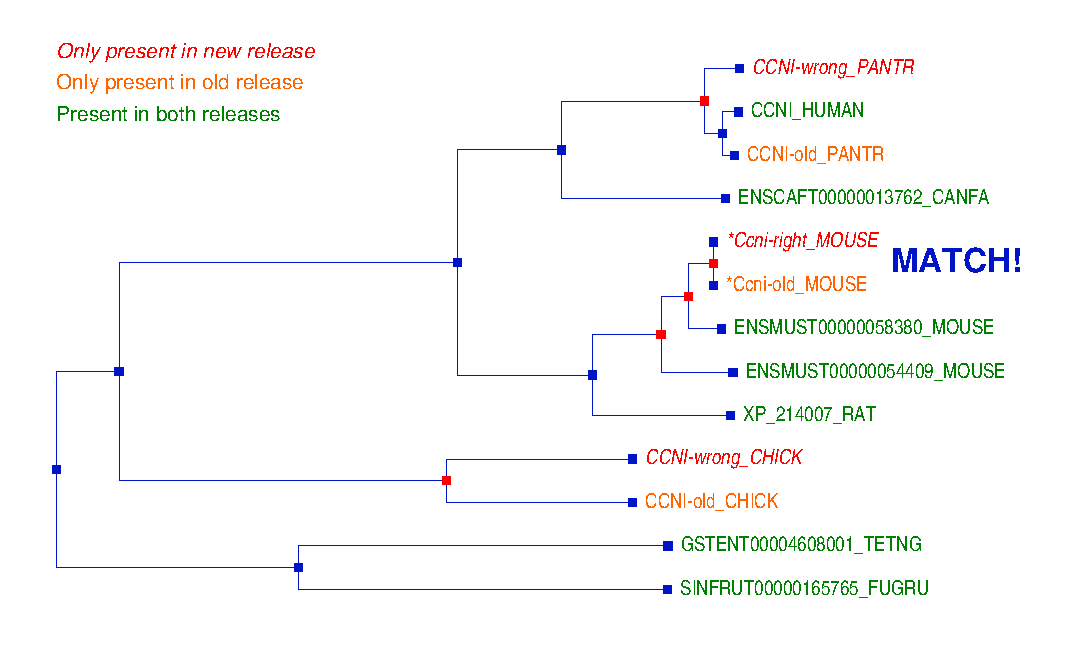
\includegraphics[width=12cm]{traceid}}}
\section{Algorithms}
\subsection{Reordering Leaves}
\frame {\includegraphics[width=10cm]{mpfig.5}}
\frame {\includegraphics[width=10cm]{mpfig.6}}
\frame {
	\frametitle{Reordering Leaves: Algorihtm}
	\begin{itemize}
	\item Goal: draw a tree in the way that minimizes $\sum_i{(i-w_i)^2}$ where
		$w_i$ is the weight of $i$-th leaf shown in the image of the tree.
	\item Algorithm: switch the left subtree and the right one at the node where
		the average weight in the left subtree is larger than the weight in the right subtree.
	\item Time complexity: $O(N)$.
	\end{itemize}
}
\subsection{Tree Merge}
\frame {
	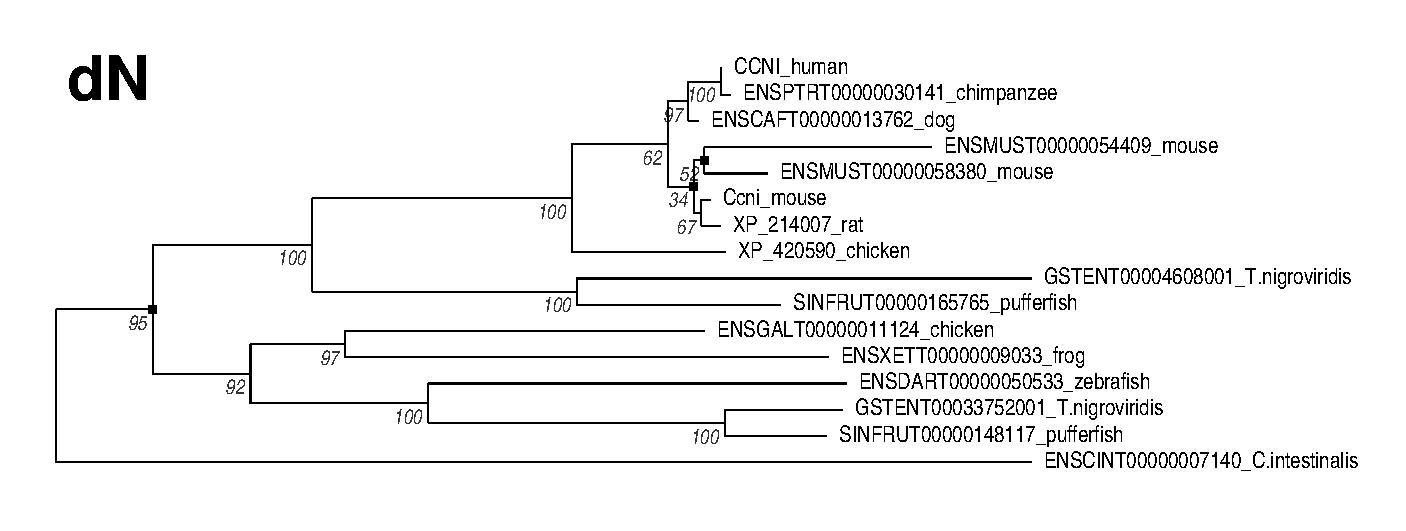
\includegraphics[width=10cm]{CCNI-dn}\\ 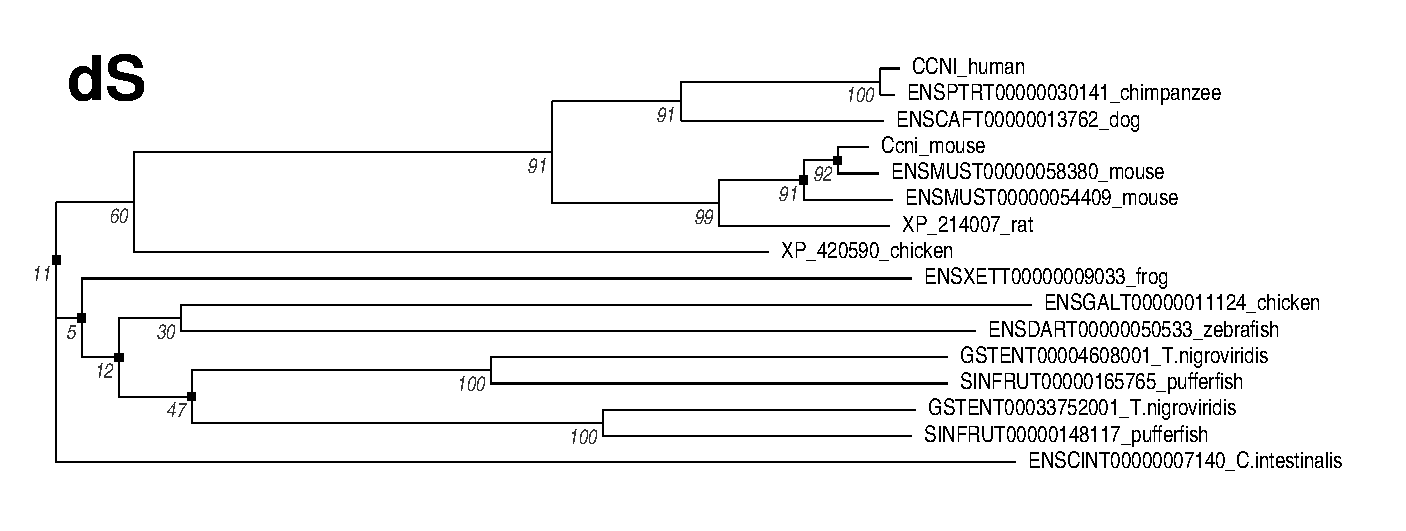
\includegraphics[width=10cm]{CCNI-ds}
}
\frame {
	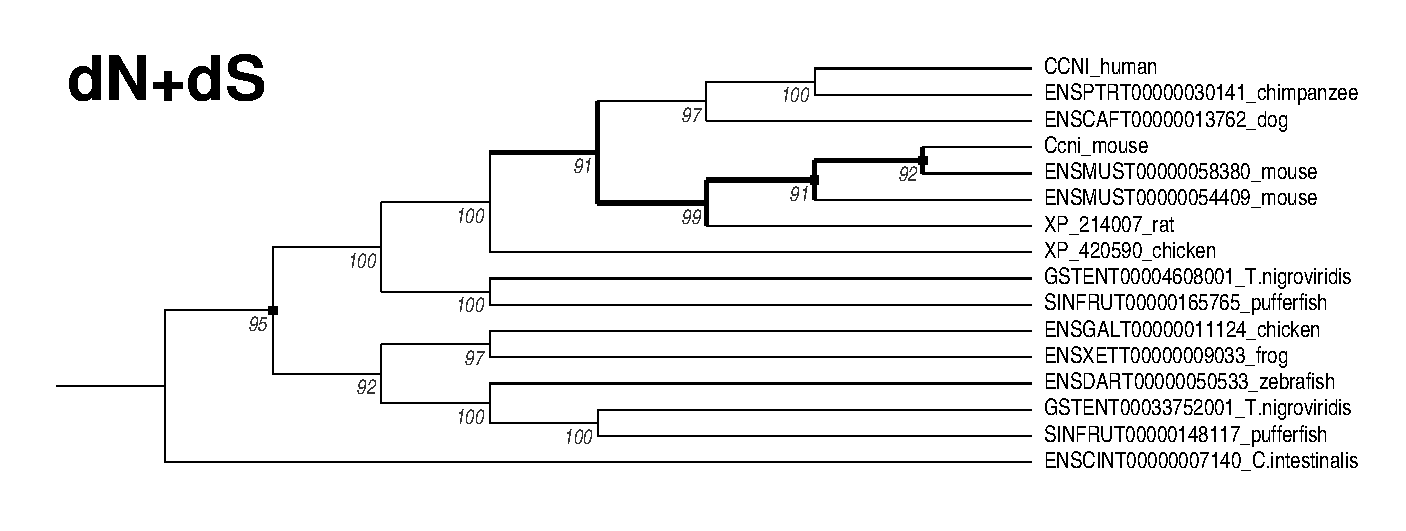
\includegraphics[width=10cm]{CCNI-dm}
}
\frame {
	\frametitle{Tree Merge: Algorithm}
	\begin{itemize}
	\item Tree merge problem: given two gene trees $G_1$ and $G_2$ which have identical leaves,
			make a merged tree $G^*$ satisfying:
		\begin{itemize}
		\item Each branch of $G^*$ comes from either $G_1$ or $G_2$.
		\item Tree $G^*$ optimizes a certain \alert{additive} objective function.
		\end{itemize}
	\item<2-> Tree merge problem can be solved in \alert{$O(N^2)$} given a class of special
			objective functions:
		\begin{itemize}
		\item Fewer duplications and losses
		\item Higher bootstrap supports
		\end{itemize}
	\item<3-> Procedures:
		\begin{itemize}
		\item Decompose trees at the branches shared by the two trees.
		\item Select the parts that optimize the objective function.
		\item Join selected parts and make the merged tree.
		\end{itemize}
	\end{itemize}
}
\frame {
	\begin{columns}
	\column{3.5cm}
	\visible{\includegraphics[height=6cm]{mpfig.1}}
	\column{8cm}
	\only<2>{\includegraphics[height=6cm]{mpfig.2}}
	\end{columns}
}
\frame {
	\begin{columns}
	\column{3.5cm}
	\visible{\includegraphics[height=6cm]{mpfig.1}}
	\column{8cm}
	\only<1>{\includegraphics[height=6cm]{mpfig.3}}
	\only<2>{\includegraphics[height=4cm]{mpfig.4}}
	\end{columns}
}
\section{New Features}
\frame {
	\frametitle{New Data}
	\begin{itemize}
		\item Expressional data (from UCSC, which has done a lot of work)
		\item Taxonomy browser
		\item Mapping traits (phenotypes from knock-out screen and nerver system functions)
		\item Choose subtree
		\item Add GO term
		\item New genomes (e.g. Build37, {\it Daphnia pulex})
		\item Ortholog
	\end{itemize}
}
\frame {
	\frametitle{New Features and Bug-Fixes}
	\begin{itemize}
		\item TreeFam API (Java API?)
		\item Multifurcated nodes ({\it Eutheria})
		\item Wiki
		\item Dead links
		\item Notung 2.1 (rearrangement seems to be a good idea)
		\item A simple list of Pfam hits
		\item What to put in CVS?
		\item Advertisement?
	\end{itemize}
}
\end{document}
